\documentclass{sigchi}

% Use this command to override the default ACM copyright statement (e.g. for preprints). 
% Consult the conference website for the camera-ready copyright statement.


%% EXAMPLE BEGIN -- HOW TO OVERRIDE THE DEFAULT COPYRIGHT STRIP -- (July 22, 2013 - Paul Baumann)
% \toappear{Permission to make digital or hard copies of all or part of this work for personal or classroom use is 	granted without fee provided that copies are not made or distributed for profit or commercial advantage and that copies bear this notice and the full citation on the first page. Copyrights for components of this work owned by others than ACM must be honored. Abstracting with credit is permitted. To copy otherwise, or republish, to post on servers or to redistribute to lists, requires prior specific permission and/or a fee. Request permissions from permissions@acm.org. \\
% {\emph{CHI'14}}, April 26--May 1, 2014, Toronto, Canada. \\
% Copyright \copyright~2014 ACM ISBN/14/04...\$15.00. \\
% DOI string from ACM form confirmation}
%% EXAMPLE END -- HOW TO OVERRIDE THE DEFAULT COPYRIGHT STRIP -- (July 22, 2013 - Paul Baumann)


% Arabic page numbers for submission. 
% Remove this line to eliminate page numbers for the camera ready copy
\pagenumbering{arabic}

% Load basic packages
\usepackage{tabularx} 
\usepackage{balance}  % to better equalize the last page
\usepackage{graphics} % for EPS, load graphicx instead
\usepackage{times}    % comment if you want LaTeX's default font
\usepackage{url}      % llt: nicely formatted URLs

% llt: Define a global style for URLs, rather that the default one
\makeatletter
\def\url@leostyle{%
  \@ifundefined{selectfont}{\def\UrlFont{\sf}}{\def\UrlFont{\small\bf\ttfamily}}}
\makeatother
\urlstyle{leo}


% To make various LaTeX processors do the right thing with page size.
\def\pprw{8.5in}
\def\pprh{11in}
\special{papersize=\pprw,\pprh}
\setlength{\paperwidth}{\pprw}
\setlength{\paperheight}{\pprh}
\setlength{\pdfpagewidth}{\pprw}
\setlength{\pdfpageheight}{\pprh}

% Make sure hyperref comes last of your loaded packages, 
% to give it a fighting chance of not being over-written, 
% since its job is to redefine many LaTeX commands.
\usepackage[pdftex]{hyperref}
\hypersetup{
pdftitle={SIGCHI Conference Proceedings Format},
pdfauthor={LaTeX},
pdfkeywords={SIGCHI, proceedings, archival format},
bookmarksnumbered,
pdfstartview={FitH},
colorlinks,
citecolor=black,
filecolor=black,
linkcolor=black,
urlcolor=black,
breaklinks=true,
}

% create a shortcut to typeset table headings
\newcommand\tabhead[1]{\small\textbf{#1}}

% shortcut for stakeholder table
\newcommand{\stakeholdertable}{
\begin{table*}
  \centering
  	\begin{tabularx}{0.9\textwidth}{|X|X|X|X|}
    \hline
    \tabhead{Direct Stakeholders} & \tabhead{Benefits/Harms} & \tabhead{Values} & \tabhead{Conflicts} \\
    \hline
    System managers & 
		\underline{Benefits}: Able to fix problems more quickly\newline
		\underline{Benefit or harm}: Less time doing maintenance and tending plants by hand\newline
		\underline{Harm}: Could be alerted of emergencies at any time
	&	Human welfare\newline
	 	Autonomy\newline
		Calmness\newline
		Free time away from work\newline
		Interaction with nature\newline
		Physical interaction with systems\newline
		Awareness (of system functioning)
	& Physical interaction with systems and awareness may conflict with calmness and free time away from work \\
    \hline
	Owners of system &
		\underline{Benefits}: System reduces labor and maintenance costs\newline
		Produce organic and high quality food\newline
		\underline{Harms}: Could suffer financial loss if system breaks down
	&	Ownership and property\newline 
		Efficiency 
	& \\
    \hline
    \hline
    \tabhead{Indirect Stakeholders} & \tabhead{Benefits/Harms} & \tabhead{Values} & \tabhead{Conflicts} \\
    \hline
    Restaurants and\newline restaurant customers &
		\underline{Benefits}: Know about where their food comes from\newline
		Provide feedbacks or improvements to owner\newline
		\underline{Harms}: Could be lied to if presented with false information
	&	Trust\newline
		Accountability\newline
		Environmental sustainability\newline
		Autonomy\newline
		Ownership and property (restaurants)
	&	Ownership and property (in the form of profitability) may compete with environmental sustainability\\
    \hline
  \end{tabularx}
  \caption{Paired down list of stakeholders}
  \label{tab:stakeholders}
\end{table*}}

% End of preamble. Here it comes the document.
\begin{document}

\title{Developing an Aquaponics Interface}

\numberofauthors{3}
\author{
  \alignauthor Justin Bare\\
    \affaddr{University of Washington}\\
    %\email{e-mail address}\\
  \alignauthor Laurel Hart\\
    \affaddr{University of Washington}\\
    \email{hart1a@uw.edu}\\
  \alignauthor Sam Wilson\\
    \affaddr{University of Washington}\\
    %\email{e-mail address}\\
}

\maketitle

\begin{abstract}
Abstract.
\end{abstract}

\keywords{
	Aquaponics; sustainability; value sensitive design;
}

\category{H.5.2.}{Information Interfaces and Presentation}{User Interfaces}

\section{Introduction}

Introduction

\section{Related Work}
\subsubsection{Aquaponics}
See Figure~\ref{fig:skales}.

\begin{figure*}[!h]
\centering
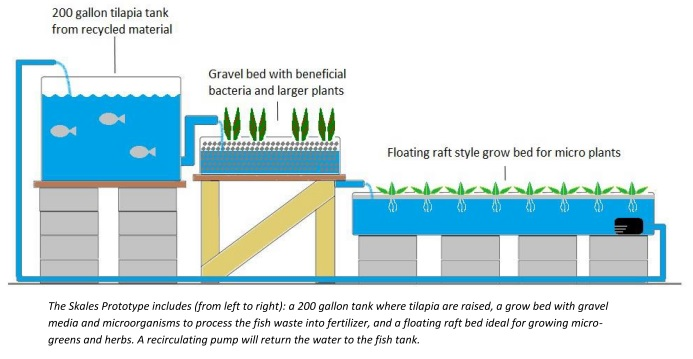
\includegraphics[width=0.9\textwidth]{systemDiagram}
\caption{Skales Cooperative aquaponics system}
\label{fig:skales}
\end{figure*}

\subsubsection{Value Sensitive Design}
Blah~\cite{VSD}

\section{Methods}

Intro to methods

\subsection{Value Sensitive Design}

Some stuff about VSD

Although we identified an extensive list of potential stakeholders, we decided to focus on only a few principle ones (see Table~\ref{tab:stakeholders}). 
\stakeholdertable

\subsubsection{Direct Stakeholders}

\subsubsection{Indirect Stakeholders}

\subsection{Iterative Design}
\begin{figure}[!h]
\centering
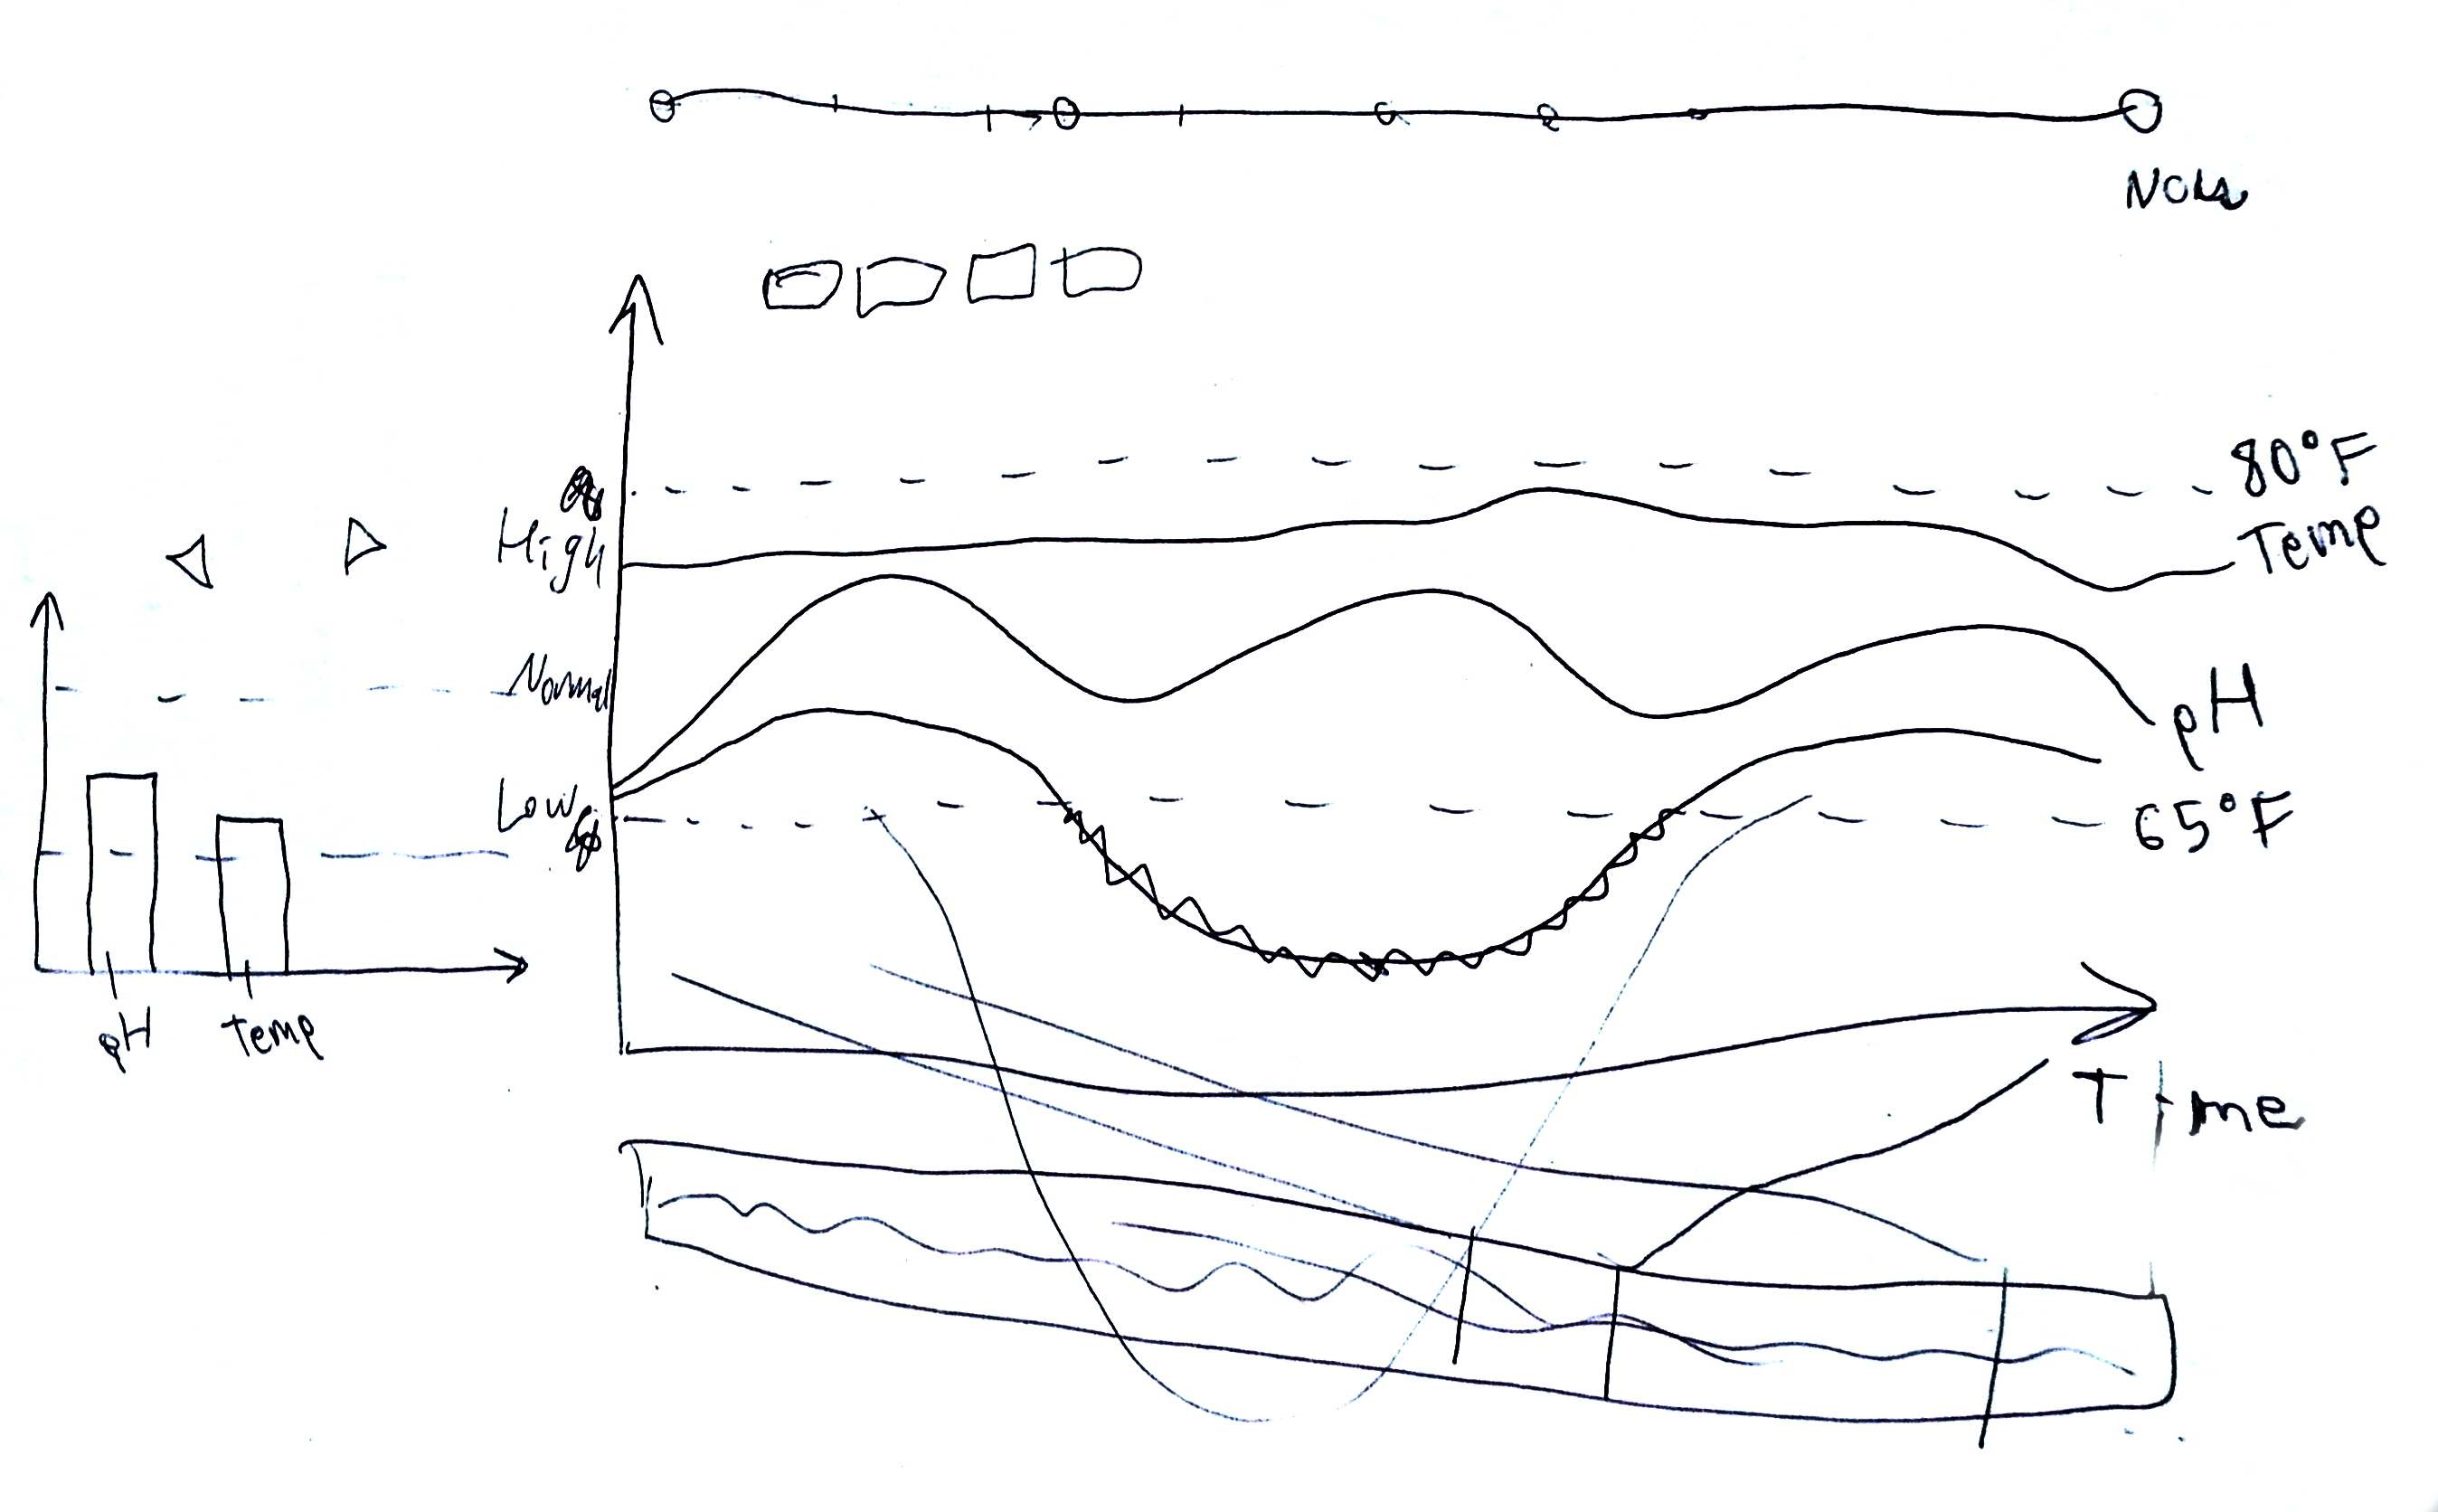
\includegraphics[width=0.9\columnwidth]{Sketch1}
\caption{Initial sketch in response to system operator's desire to see all information at a glance.}
\label{fig:sketch1}
\end{figure}

\begin{figure}[!h]
\centering
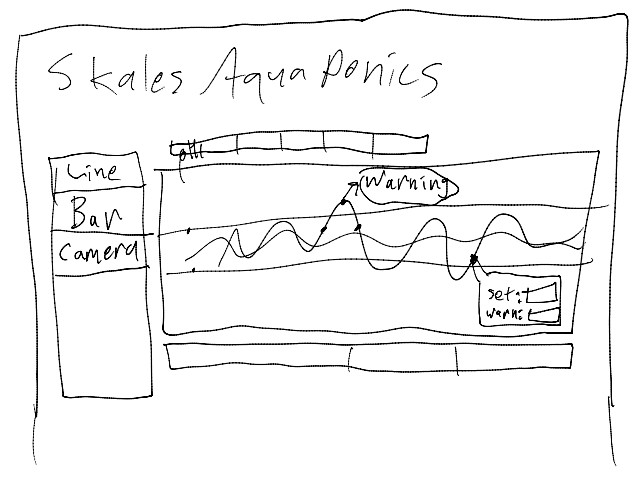
\includegraphics[width=0.9\columnwidth]{Sketch2}
\caption{Refinement upon first sketch.}
\label{fig:sketch2}
\end{figure}

\begin{figure*}[!h]
\centering
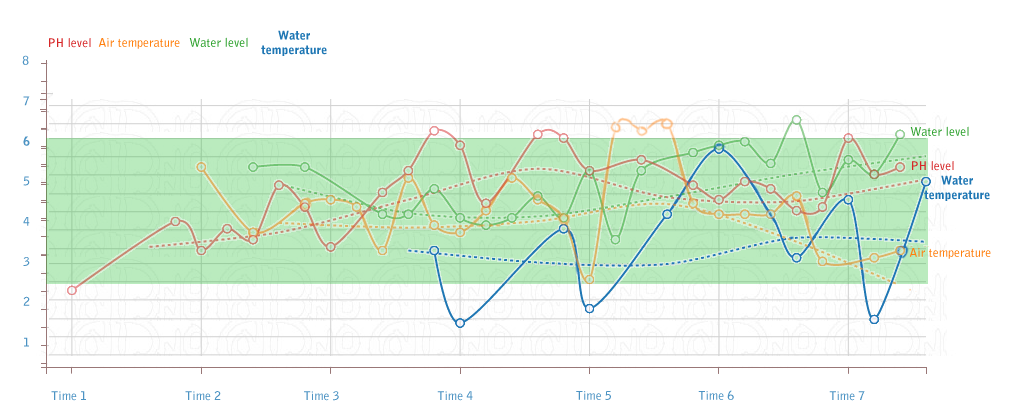
\includegraphics[width=0.9\textwidth]{Mockup}
\caption{Color mockup based on D3.js aesthetics.}
\label{fig:mockup}
\end{figure*}

D3.js: \cite{d3js}
 
\section{Results}

Blah

\section{Conclusion}

Blah

\section{Future Work}

\subsubsection{Additional Stakeholders}
Fish

% Balancing columns in a ref list is a bit of a pain because you
% either use a hack like flushend or balance, or manually insert
% a column break.  http://www.tex.ac.uk/cgi-bin/texfaq2html?label=balance
% multicols doesn't work because we're already in two-column mode,
% and flushend isn't awesome, so I choose balance.  See this
% for more info: http://cs.brown.edu/system/software/latex/doc/balance.pdf
%
% Note that in a perfect world balance wants to be in the first
% column of the last page.
%
% If balance doesn't work for you, you can remove that and
% hard-code a column break into the bbl file right before you
% submit:
%
% http://stackoverflow.com/questions/2149854/how-to-manually-equalize-columns-
% in-an-ieee-paper-if-using-bibtex
%
% Or, just remove \balance and give up on balancing the last page.
%
\balance

\bibliographystyle{acm-sigchi}
\bibliography{FinalProjectReport}
\end{document}
